\documentclass[a4paper, 12pt]{article}
%\documentclass[a4paper, 12pt, draft]{article} % don't include images, leave a border of same size...great


%\usepackage[cmex10]{amsmath, mathtools}
\usepackage{amsmath,amssymb,amsbsy,amsfonts,amsthm}
\usepackage{bm}
\usepackage{enumerate}
\usepackage{url}
\usepackage[ruled,vlined]{algorithm2e}
\usepackage{fancyvrb}
\usepackage{yfonts}
\usepackage{multirow}
\usepackage{multicol}
\usepackage[margin=6.5em]{geometry}


\usepackage{wrapfig}
\usepackage{tikz}
%\input{../tikz.conf}

\usetikzlibrary{bayesnet}

%%%%%%%%%%% Box 
\usepackage{calc}%    For the \widthof macro
\usepackage{xparse}%  For \NewDocumentCommand
\newcommand{\tikzmark}[1]{\tikz[overlay,remember picture] \node (#1) {};}


%\input{./header.tex}
%%%%%%%%%% Math
\renewcommand{\text}{\textnormal}
%\newcommand{\pr}{\mathbf{p}}
\newcommand{\pr}{p}
\newcommand{\p}{p}
\newcommand{\E}{\mathbb{E}}
\newcommand{\divkk}{\mathbb{K}}
\newcommand{\entropy}{\mathbb{H}}
\newcommand{\gem}{\mathrm{GEM}}
\newcommand{\Mult}{\mathrm{Mult}}
\newcommand{\DP}{\mathrm{DP}}
\newcommand{\IBP}{\mathrm{IBP}}
\newcommand{\M}{\mathcal{M}}
\newcommand{\V}{\mathcal{V}}
\newcommand{\N}{\mathcal{N}}
\renewcommand{\L}{\mathcal{L}}
\newcommand{\mat}[1]{\mathbf{#1}}
\newcommand{\unit}{1\!\!1}
\newcommand{\zij}{z_{i\rightarrow j}}
\newcommand{\zji}{z_{i\leftarrow j}}

%\renewcommand{\Phi}{\mat{\Phi}}

\title{Mixed-Membership Inference in Sparse Weigted Networks.}

%\date{avril 2015}

\newtheorem{definition}{Definition}[section]
\newtheorem{proposition}{Proposition}[section]
\newtheorem{theorem}{Theorem}[section]
\newtheorem{corollary}{Corollary}[section]

\begin{document}
	
\maketitle
\begin{abstract}
\end{abstract}



\section{Introduction}

Link prediction in networks is a well-known problem that has been addressed by many studies, as \cite{Liben2007,Zaki2011,Martinez2016} for social networks. If knowing that a link relates two nodes in a network is important, the intensity of each link plays a major role in many situations. For example, in epidemiology, the number of contacts between two persons is an important factor to accurately estimate the probability of contagion between from one person to the other. Similarly, to understand the population dynamics between two cities, it is not sufficient to knwow that there is a motorway or an airline relating them, it is also necessary to know the number of vehicles or passengers that transit between them. In the fields of economy and finance, to estimate whether a company will be controlled by another company which has recently acquired part of its shares, it is important to know the actual number of shares acquired. In all these examples, the relations between the entities involved (persons, cities, companies) can be modeled by weighted graphs, in which entities correspond to nodes and relations (contacts between persons, transport connections between cities and acquisitions between companies) to links. The weight on each link represents the intensity of the relationship between the nodes. Furthermore, if the weights can sometimes take both positive and negative values, as in \textit{signed} social networks \cite{Kumar2016} for representing approval/disapproval, like/dislike or trust/distrust, most weighted networks rely on positive integers. The prevalence of this type of networks may be explained by the fact that many weighted networks are the results of the superposition, over time, of atomic, binary interactions (the well-known Enron email network, for example, is weighted according to the number of emails exchanged between Enron employees, the atomic interaction being the exchange of the single email).

Two main approaches have been proposed to solve the weight prediction problem \cite{Lu2011} in networks. In the first type of approaches, one finds methods that assume that the weight of a link is correlated with the similarity between the nodes of the link, this similarity being based on neighboring nodes \cite{Zhao2015,Zhu2016}. If the assumption \textit{a node behaves like its neighbors} is used, to different extent, in network studies, it is however not sufficient to explain all the observed interactions between nodes. Several researchers have thus adopted a second type of approach, based on generative models within well-defined probabilistic frameworks. Such models aim at making explicit how links, and their weights, are produced. Among such generative models, stochastic block models and their extensions through mixed-membership stochastic block models have received particular attention \cite{ Karrer2011,airoldi2009mixed,iMMSB,fan2015dynamic} as they can account for the underlying classes that structure real-world networks and in particular social networks. Nevertheless, most models proposed so far have been devoted to unweighted networks and, to our knowledge, only two models in the stochastic block model family have been proposed for weighted graphs: The latent block structure model of \cite{aicher2014learning} and the weighted stochastic block model of \cite{peixoto2018nonparametric}. These two models however suffer from the same drawback as standard stochastic block models, namely the fact that a node can belong to only one class, which is not realistic for many networks. Mixed-membership block models were specifically designed to overcome this limitation and we propose here a new mixed-membership block model adapted to weighted networks. Our contributions are in fact twofold:
%
\begin{enumerate}
\item We propose the first, to our knowledge, mixed-membership stochastic block model for weighted networks where weights are positive integers.
\item We show how, by combining several state-of-the-art methods, one can deploy such methods on large networks.
\end{enumerate}
%
The remainder of the paper is organized as follows: Section~\ref{sec:rl} describes related work; Section~\ref{sec:model} then presents the weighted mixed-membership stochastic block model we retained while Section~\ref{sec:inference} details its inference. Section~\ref{sec:exps} illustrates the behavior of the proposed models on several real-world networks. Finally, Section~\ref{sec:concl} concludes the study.


%From social networks to protein interactions, from physics to linguistics, networks are one of the key representations for objects interacting with one another. The interest for modeling such networks has naturally increased with the availability of large datasets, and people have tried to design generative models to describe the formation of links between nodes. Among such generative models, stochastic block models and their extensions through mixed-membership block models have received particular attention \cite{airoldi2009mixed,iMMSB,fan2015dynamic} as they can account for the underlying classes that structure real-world networks and in particular social networks. Nevertheless, most models proposed so far are devoted to unweighted networks. To our knowledge, only two models, in the stochastic block model family, have been proposed for weighted graphs: the latent block structure model of \cite{aicher2014learning} and the weighted stochastic block model of \cite{peixoto2018nonparametric}. These two models however suffer from the same drawback as standard stochastic block models, namely the fact that a node can belong to only one class, which is not realistic for many networks. Mixed-membership block models were specifically designed to overcome this limitation and we propose here a new mixed-membership block model adapted to weighted networks. One important aspect in designing a generative model for networks is to develop a scalable inference method so that the model can be applied on large networks. We rely in this study on collapsed variational inference coupled with stochastic variational inference to do so.


\section{Weighted Networks and Time exchangeability}

% dense - unrealistic
The link prediction models, in the literature \cite{goldenberg2010survey,lu2011link}, usually represent a network by a graph $G=(V,E)$, where $V$ is a set of vertex and $E$ a set of edges between the vertex. It can be represented by its adjacency matrix $(Y_{ij})_{(ij) \in V^2} \in \mathcal{Y}$. For a binary network, the support of the edges is $\mathcal{Y} = (0,1)$ to account respectively for the absence or the presence of an edge between two nodes. Formally the likelihood of such model is characterized by a Bernoulli density such that $y_{ij} \sim \mathrm{Bern}(\theta)$. If $\theta$ is a constant, this is an Erd\"o-R\'eniy model. Relaxing this unrealistic assumptions with a latent model gives the Stochastic Blockmodel, and more recently, by relaxing the hard assignment to blocks, gives the Mixed-Membership Stochastic Blockmodel (MMSB) \cite{MMSB}. Moreover all of those models are in a setting of binary networks and  static graphs which is formally traduced by an assumption of exchangeability. It means that the joint probability of a graph do not depend on the order of which we observes the nodes. %? $echangeability$

\textcolor{red}{\paragraph{cette sous section sur la sparsite a revoir et aligner avec les update SCVB ! The weighted model is still exchangeable ?}~\\
% sparse - real
The main limitation of such models is that they can't handle sparse networks, which is a corollary of the Aldous-Hoover theorem \cite{orbanz2015bayesian}. The models has been said to be misspecified. A way to alleviate this limitation is to weight edges instead of considering binary one. This weighting can be understood, in some way, as smoothing the networks. Additionally, a weighted network is a binary networks where information has bee added under the for of node labeling. The reason why sparsity could be handle this way is because, by considering a weighted networks, it makes all non-edges in a network (0 entries in the adjacency matrix) having a weak contribution to the degree distribution of associated node (see section \ref{todo}). Thus, the inference process can take advantage of this fact because, in sparse networks, most of the interactions are unrealized.}

In this paper we will consider the weighted relations as a measure for the number of times each nodes have interacted. Thus, a natural prior for such assumptions is a Poisson distribution. It follows that we will define the likelihood to generate a weighted edge such that $y_{ij} \sim \mathrm{\theta_{ij})}$. Moreover, this representation can take advantage of relational data that arise in various scenario, summarized by the two following:
\begin{itemize}
\item Weighted Networks, where weights represent the \emph{strength} of the relations between individuals,
\item Sum of \emph{snapshot} of binary (or weighted) networks.
\end{itemize}

In the second case the weights can also be seen as a \emph{strength} of connection between individuals, since it represents a count/number of times they interacted together. There is a number of situations where such a case arise. One can think for example, to the count of clicks that an user makes during a web session. Or the number of time that a individual send a message to another in a communication network, such as email or online social networks. Or again, the number of transportation between two cities. Thus modeling weighted networks is a way to take into account the strength of relations that arise in a temporal context, but by keeping the exchangeability assumptions. Or says differently, we loose the time order in which each individual connections took place. That is the reason why we use the term \emph{time exchangeability}.

The use of a Poisson law as an aggregator for single snapshots is primarily justified by the two following fundamental properties \cite{orbanz2015bayesian}:
\begin{itemize}
\item{Additivity}: If $K_1 \sim \mathrm{Poisson}(\alpha_1)$ and $K_2 \sim \mathrm{Poisson}(\alpha_2)$ then:
    \begin{equation}
        K_1 + K_2 = \mathrm{Poisson}(\alpha_1 + \alpha_2)
    \end{equation}
\item {Thinning}: The number of successes in a Poisson number of coin flips is Poisson, namely if $K \sim \mathrm{Poisson}(\alpha)$ and $X_1,...,X_2 \sim_{iid} \mathrm{Bern}(p)$, then:
    \begin{equation}
        \sum_{i=1}^K X_i = \mathrm{Poisson}(p\alpha)
    \end{equation}
\end{itemize}

Those two properties of the Poisson distribution constitute the justification of building weighted networks datasets from sequence of either weighted graphs or binary graphs and making inference with Poisson based likelihood.

Those two properties gives us a justification for building and model weighted networks with a Poisson kernel, from sequence of snapshot, of either binary or weighted, networks. 

\section{Model -- WMMSB}
A powerful model for binary exchangeable networks is the Mixed Membership Stochastic Blockmodel (MMSB). In order to keep the strength behind the MMSB models, we propose a generalization of it for weighted networks such as described in the previous section.

The proposed model is a weighted extension of MMSB, named WMMSB. The main design difference is that the likelihood is drawn from a Poisson distribution, and the correlations between the shared classes are drawn from independent Gamma distributions. The model first draw latent class membership for each node from a shared Dirichlet distribution. Then for each interactions,  nodes draw a single membership. The observation level is then draw from Poisson distribution taking its rate parameter according to two classes that summarize the interaction between the two underlying nodes. The observation corresponds to the strength of the relationship between two classes. The generative model (along  with the graphical model) is summarized as follows:

\begin{figure}[h]
    \hspace*{-3.7em}
\begin{minipage}[h]{0.3\linewidth}
\begin{align*}
	&\textrm{For each } i \in \{1, .., N\}  \\
	&\qquad\bm{f}_i \sim \textrm{Dir}(\alpha)\\
	&\textrm{For each }  (m,n) \in \{1,..,K\}^2 \\
	&\qquad\phi_{mn} \sim \mathrm{Gamma}(\eta,\theta)\\
	&\textrm{For each } (i,j) \in V^2 \\
	&\qquad z_{i \rightarrow j} \sim \mbox{Cat}(\bm{f}_i)\\
	&\qquad z_{i \leftarrow j} \sim \mbox{Cat}(\bm{f}_j)\\
    &\qquad y_{ij} \sim \mathrm{Poisson}(\phi_{z_{i \rightarrow j}z_{i \leftarrow j}})
\end{align*}
\end{minipage}
\begin{minipage}[h]{0.3\linewidth}
	\scalebox{0.88}{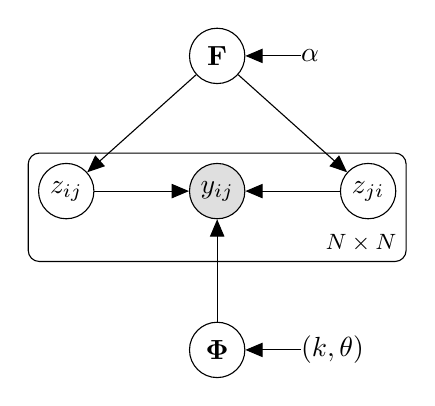
\begin{tikzpicture}
    %\begin{scope}[yshift=0.5cm]
  % Define nodes
  \node[obs]                      (y) {$y_{ij}$};
  \node[latent, left=1.2cm of y] (zi) {$z_{ij}$};
  \node[latent, right=1.2cm of y] (zj) {$z_{ji}$};
  \node[latent, above= of y]    (ibp) {$\mat{F}$};;
  \node[latent, below= of y, yshift=-0.3cm]   (W) {$\mat{\Phi}$};
  \node[const, right=0.7cm of ibp]   (b) {$\alpha$};
  \node[const, right=0.7cm of W]   (sw) {($k,\theta$)};

  % Connect the nodes
  \edge {zi,zj,W} {y} ;
  \edge {ibp} {zi,zj} ;
  \edge {sw} {W} ; 
  \edge {b} {ibp} ; 

  % Plates
  \plate {yx} {(zj)(zi)(y)} {$N\times N$} ;
  %\end{scope}
\end{tikzpicture}
}
\end{minipage}
    \caption{Generative models and Bayesian graph of WMMSB.}
\end{figure}

Note that the group membership of each node is context dependent. That is, each node may assume different membership when interacting or being interacted with by different peers. Statistically, each node is an admixture of group-specific interactions. The two sets of latent group indicators are denoted by $Z_\rightarrow = \{z_{p\rightarrow q} : p, q \in V\}$ and $Z_\leftarrow = \{z_{p\leftarrow q} : p, q \in V\}$. Also note that the correlation between classes need not be equal. Equality may be enforced when modeling symmetric interactions. \cite{goldenberg2010survey}.

%In the rest of this paper  we will note the set of hyperparameters as $\H = (\alpha, \theta, k)$.

For simplicity, the marginal likelihood (or evidence), takes the following form:
\begin{equation}
    \p(Y | \alpha, \Phi) = \int_F \sum_Z \p(Y| Z, \Phi) \p(Z|F) \p(F| \alpha) dF
\end{equation}

Furthermore, observed links are conditionally independent given the parameters for nodes ($F$) and for classes ($\Phi$) and by marginalizing over the class membership. Thus the likelihood can be written as a matrix decomposition :
\begin{equation}
P(Y | F, \Phi) = \prod_{i,j \in V^2} f_i \Phi f_j^T
\end{equation} 

Unfortunately the evidence is intractable, and conducts the practitioner to resort to approximate inference. In the next section, we propose a Stochastic Collapsed Variational inference method.

\section{Inference}


\subsection{Collapsed Variational Inference}

The Variational Bayes (VB) method is an inference method based on the approximation of the Bayesian model's parameters, $(F, \Phi, Z)$, with free variational parameters $(\nu, \epsilon, \gamma)$ usually taken in the same family than the true parameters. It consists of an iterating algorithm which updates the variational parameters by maximizing the lower bound arising from the Jensen Inequality. This is equivalent to  minimize the Kullback-Leibler divergence between the variational (posterior) distribution over the variational parameters denoted $q(F, \Phi, Z | \nu, \epsilon, \gamma)$ (we will suppress reference to the variational parameters in the variational posterior for brevity) and the true (posterior) distribution $p(F, \Phi, Z | \tau)$ where $\tau = (\alpha, \eta, \theta)$ denotes the set of hyperparameters of the model. The evidence lower bound (ELBO) takes the following form :

\begin{align}
    \log p(Y | \tau) &\geq \mathcal{L}(q(F, \Phi, Z)) \\
    &= E_q[\log p(Y, F, \Phi, Z | \tau)] - E_q[\log q(F, \Phi, Z)] \nonumber \nonumber
\end{align}

In classical VB, the variational parameters are taken in the same family than the true parameters and by assuming that they are fully independent, this is know as the mean-field approximation :
\begin{equation}
q(F, \Phi, Z) = \prod_{i\in V}q(f_i | \nu_i) \prod_{k,k' \in K^2}q(\phi_{kk'} | \epsilon_{kk'})\prod_{i,j \in V^2}q(\zij, \zji | \gamma_{ij})
\end{equation}

In the Collapsed Variational Bayes (CVB), the assumption on the variational distribution is much weaker and therefore constitute a better approximation than standard VB \cite{teh2006collapsed}. We only assume that the $Z$ variables are mutually independent, then the variational posterior becomes : 
\begin{align}
q(F, \Phi, Z) &= q(F,\Phi) \prod_{(i,j)\in V^2}q(\zij, \zji | \gamma_{ij}) \\
	&= q(F, \Phi | Z)q(Z)
\end{align}

The ELBO can be split by separating both independent contributions of the variational posterior. Since we do not restrict the form of $q(F, \Phi | Z)$, the ELBO maximum is achieved when the true posterior is reached at $p(F, \Phi | Y, Z,  \tau) = q(F, \Phi | Z)$. The ELBO simplifies in the following collapsed form :
\begin{align}
    \mathcal{L}(q(Z)) &= \max_{q(F,\Phi|Z)} \mathcal{L}(q(F, \Phi|Z)q(Z)) \\
    &= E_q[\log p(Y,Z|\tau)] - E_q[q(Z)]
\end{align}

The variational parameters are chosen in the same family of distribution than the true distribution, thus $q(\zij=k, \zji=k' | \gamma_{ij})$ are multinomial with parameters $\gamma_{ij}$.

Finally, the CVB update is obtained by maximizing the collapsed ELBO with respect to $\gamma_{ijkk'}$ and it takes the following general form :
\begin{equation} \label{eq:cvb_update}
    \gamma_{ijkk'} \propto \exp \left( E_{q(Z^{\neg ij})} [\log(\zij=k, \zji=k' |Y, Z^{\neg ij}, \tau)] \right)
\end{equation}

Where the superscript $\neg ij$ means that the corresponding variables (or counts) are excluded.
This equation is not directly tractable, therefore it is possible to approximate equation \eqref{eq:cvb_update} by noting its relation with the collapse Gibbs update. Then,  the closed form expression for the CVB update can be obtained by using a central limit theorem approximation followed by a Taylor expansion.

The Collapse Gibbs Sampler (CGS) for both models are given by the following update rule :

%\begin{align} \label{eq:post_cgs}
%    p(\zij=k, \zji=k' | Y, Z^{\neg ij}, \tau) \propto  \quad & p(y_{ij} | Y^{\neg ij}, Z^{\neg ij}, \zij=k, \zji=k', \tau) \nonumber\\
%    & p(\zij=k, \zji=k' | Z^{\neg ij}, \tau)
%\end{align}
\begin{align} \label{eq:post_cgs}
    &p(\zij=k, \zji=k' | Y, Z^{\neg ij}, \tau) \propto  \nonumber\\
    & \quad p(\zij=k, \zji=k' | Z^{\neg ij}, \tau) \nonumber \\
    & \quad p(y_{ij} | Y^{\neg ij}, Z^{\neg ij}, \zij=k, \zji=k', \tau)
\end{align}

Both MMSB and WMMSB models had in common the prior over the latent classes which characterise the mixed-membership effect. The update for the left hand part of equation \eqref{eq:post_cgs} represents a reinforcement effect on latent classes membership :

\begin{align}
    & p(\zij=k, \zji=k' | Z^{\neg ij}, \tau) \propto  \nonumber\\
    & (n^{F\neg j}_{ik} + \alpha_k) (n^{F\neg i}_{jk} + \alpha_{k'}) 
\end{align}


Both models difference arise from their kernels that are respectively Bernoulli-Beta and Poisson-Gamma distributed for MMSB and WMMSB. The righ part of equation \eqref{eq:post_cgs} are given by the following equations :

\begin{itemize}
    \item MMSB : {\setlength{\mathindent}{0cm} \begin{align} \quad & p(y_{ij} | Y^{\neg ij}, Z^{\neg ij}, \zij=k, \zji=k', \tau) = \nonumber \\ & \quad  \frac{ n^{\Phi\neg ij}_{y_{ij}kk'} + \lambda_{y_{ij}}}{n^{\Phi\neg ij}_{\bm{.}kk'} + \lambda_{\bm{.}}}\end{align}}
        \item WMMSB : {\setlength{\mathindent}{0cm} \begin{align} &\quad p(y_{ij} | Y^{\neg ij}, Z^{\neg ij}, \zij=k, \zji=k', \tau) = \nonumber\\& \quad  NB(y_{ij}; n^{Y\neg ij}_{kk'} + \eta, \frac{1}{n^{\Phi\neg ij}_{\bm{.}kk'} + \theta + 1} )\end{align}}
\end{itemize}

Where $NB(x;a, b)$ represents the pdf of a Negative Binomial distribution parametrized by $(a,b)$.

The collapse Gibbs Samplers only need to update the various counts $n^*$ that emerge from the conjugacy of prior in the *MMSB models. The counts represents the following quantities :
%\begin{align}
%    &n^{F}_{ik} = \sum_j \delta(\zij=k) + \delta(z_{j\leftarrow i}=k) \qquad\qquad\qquad n^{Y}_{kk'} = \sum_{ij} y_{ij}\delta(\zij=k, \zji=k') \\
%    &n^{\Phi}_{xkk'} = \sum_{ij} \delta(y_{ij}=x, \zij=k, \zji=k') \qquad  n^{\Phi}_{\bm{.}kk'} = \sum_x n^{\Phi}_{xkk'}
%\end{align}
\begin{align}
&n^{F}_{ik} = \sum_j \delta(\zij=k) + \delta(z_{j\leftarrow i}=k) \\  
&n^{Y}_{kk'} = \sum_{ij} y_{ij}\delta(\zij=k, \zji=k') \\
&n^{\Phi}_{xkk'} = \sum_{ij} \delta(y_{ij}=x, \zij=k, \zji=k') \\
&n^{\Phi}_{\bm{.}kk'} = \sum_x n^{\Phi}_{xkk'}
\end{align}

In order to compute equation \eqref{eq:cvb_update}, one can approximate the variational distribution with a zero Taylor expansion under a Gaussian approximation. 

By the central limit theorem, one can compute the expectations of the counts statistics under the variational distribution, that we will refer as $N^* \approx E_q[n^*]$. They are given by a sum of independent variables, where each token is the result of a Bernoulli trial with mean $\gamma_{ijkk'}$. The variational counts statistics can be obtained as follow:

\begin{align} \label{eq:stat_cvb}
    &N^{F}_{ik} = \sum_{j, k'} \gamma_{ijkk'} \qquad\quad  N^{Y}_{kk'} = \sum_{ij} y_{ij}\gamma_{ijkk'} \\
    &N^{\Phi}_{xkk'} = \sum_{ij:y_{ij}=x} \gamma_{ijkk'} \qquad  N^{\Phi}_{\bm{.}kk'} = \sum_x N^{\Phi}_{xkk'}
\end{align}

Under this Gaussian approximation, we can apply a Taylor expansion of equation \eqref{eq:cvb_update}. For simplicity and effectiveness \cite{asuncion2009smoothing}, we propose a zero order approximation, which is know as the CVB0 algorithm and gives the following updates :

\begin{itemize}
    \item MMSB : \[ \gamma_{ijkk'} \propto  \frac{ N^{\Phi\neg ij}_{y_{ij}kk'} + \lambda_{y_{ij}}}{N^{\Phi\neg ij}_{\bm{.}kk'} + \lambda_{\bm{.}}} (N^{F\neg j}_{ik} + \alpha_k) (N^{F\neg i}_{jk} + \alpha_{k'})\]
    \item WMMSB : \[ \gamma_{ijkk'} \propto NB(y_{ij}; n^{Y\neg ij}_{kk'} + \eta, \frac{1}{n^{\Phi\neg ij}_{\bm{.}kk'} + \theta + 1} ) (N^{F\neg j}_{ik} + \alpha_k) (N^{F\neg i}_{jk} + \alpha_{k'})\]
\end{itemize}

One can remark the similarity with the Collapse Gibbs update. But as the inference is deterministic, it is possible to derive a stochastic gradient in order to prevent batch learning and to scale to large datasets.

\subsection{Stochastic Variational Inference}

We propose to derive update for a Stochastic Collapsed Variational Inference (SCVB) for the *MMSB models. It is closely related to The Stochastic Variational Inference (SVB)  where online inference is made possible with variational Inference in the exponential family and to \cite{hoffman2013stochastic} which propose general online E-M algorithm for latent model \cite{cappe2009line}. This approach is useful for the two following reasons :

\begin{itemize}
    \item Scale to large datasets : The time complexity becomes linear with the size of the datasets because the algorithm can work with minibatch of an arbitrary size. The memory complexity is drastically save, because only the minibatch content need be loaded to fit a model against the quadratic complexity usually met in networks.
    \item Dynamic scenario : The size of the minibatch can be arbitrary chosen, and could be use in streaming learning scenario, by relaxing the assumptions made on the step size if the Stochastic gradient.
\end{itemize}

The CVB algorithm is resumed by the statistics $N^*$ (see equations \eqref{eq:stat_cvb}). It means that the model parameter can be recovered from those statistics :

\begin{align}
    \hat f_{ik} &= \frac{N^{F}_{ik} + \alpha_k }{2|V| + \alpha_{\bm{.}}} \\
    \hat \phi_{kk',x} &= \frac{ N^{\Phi}_{x, kk'} + \lambda_x}{N^{\Phi}_{\bm{.}, kk'} + \lambda_{\bm{.}}}  \qquad \mathrm{for}\quad\mathrm{MMSB}\\
    \hat \phi_{kk',x} &= NB(x; N^Y_{kk'} + \eta, \frac{1}{N^{\Phi}_{\bm{.}kk'} + \theta + 1} ) \qquad \mathrm{for}\quad\mathrm{WMMSB}
\end{align}

For one observations, global statistics are updated by computing the natural gradient of the objective under variational parameter and given by the following steps :
\begin{itemize}
    \item Maximization : The current state is approximately maximized from the update of $\gamma_{ij}$ which optimize the ELBO for the current token,
    \item Expectation : The expected count statistics are updated which propagates the new observations to the noisy gradient. This propagation is controlled by a gradient step size $\rho^{*}_t$ such that $N^{*, t} = (1-\rho_t)N^{*,t-1} + \rho_t \overline N^{*,t}$
\end{itemize}

Where $\overline N$ is the expected statistics computed as if all observations where drawn as the current variational parameters $\gamma_{ij}$. That is the corresponding  expectation for an observations $(ij)$  are given for the different statistics :
\begin{itemize}
    \item $\overline N^{F}_i = R_i \gamma_{ij}$ where $R_i=2|V_i|$ is the total number of relations for a node $i$ in a graph,
    \item $\overline N^{\Phi} = R Y^{(ij)}$ where $R$ is the total number of relations in the network, for a directed graph is $R=|V|^2$, and $Y^{(ij)}$ is $|\mathcal{Y}| K^2$ tensor such that the matrix entries corresponding to the index equal to $y_{ij}$ are set to $\gamma_{ij}$ and the other ones to zeros.
    \item $\overline N^Y = Ry_{ij}\gamma_{ij}$, similar statistics than  $\overline N^{\Phi}$ for weighted networks.
        
\end{itemize}

Todo :
\begin{itemize}
    \item gradient step constraint for convergence
    \item (reflexion) what does  it means in term of convergence and step gradient constraint,  if I want to forget old data, make a global burstiness effect (a sparse network) ??
\end{itemize}

Thus our algorithm is very similar than the one use by \cite{foulds2013stochastic} for their SCVB algorithm adapted for LDA and text data.

%\section{Sparsity and Preferential Attachment}

\section{Experiments}

%WMMSB compare it with LDA (a mask)i vs a bipartite networks (Document)
%D (doc) x W (Voc) -- entry count
%
%the bag of word VS the networks representation of document
%* it adds a parameter the document modelization !!!!!!!

\clearpage

\bibliographystyle{unsrt}
\bibliography{./a}

\appendix

\end{document}

